\chapter{Project setup}\label{Chap:Setup}
In this section will be described the necessary steps to have the application up and running.
\section{Necessary libraries}
The setup of the necessary libraries and framework has been done simmetrically to the one performed in DP2 virtual machine available on the course website. Only difference is the addition of Z3 library for the machine, the setup of it is shown in section \ref{SubSec:Z3Setup}. In figure \ref{Fig:OptFolder} is shown the actual setup used for the machine.
\begin{figure}[!htb]
   \centering
   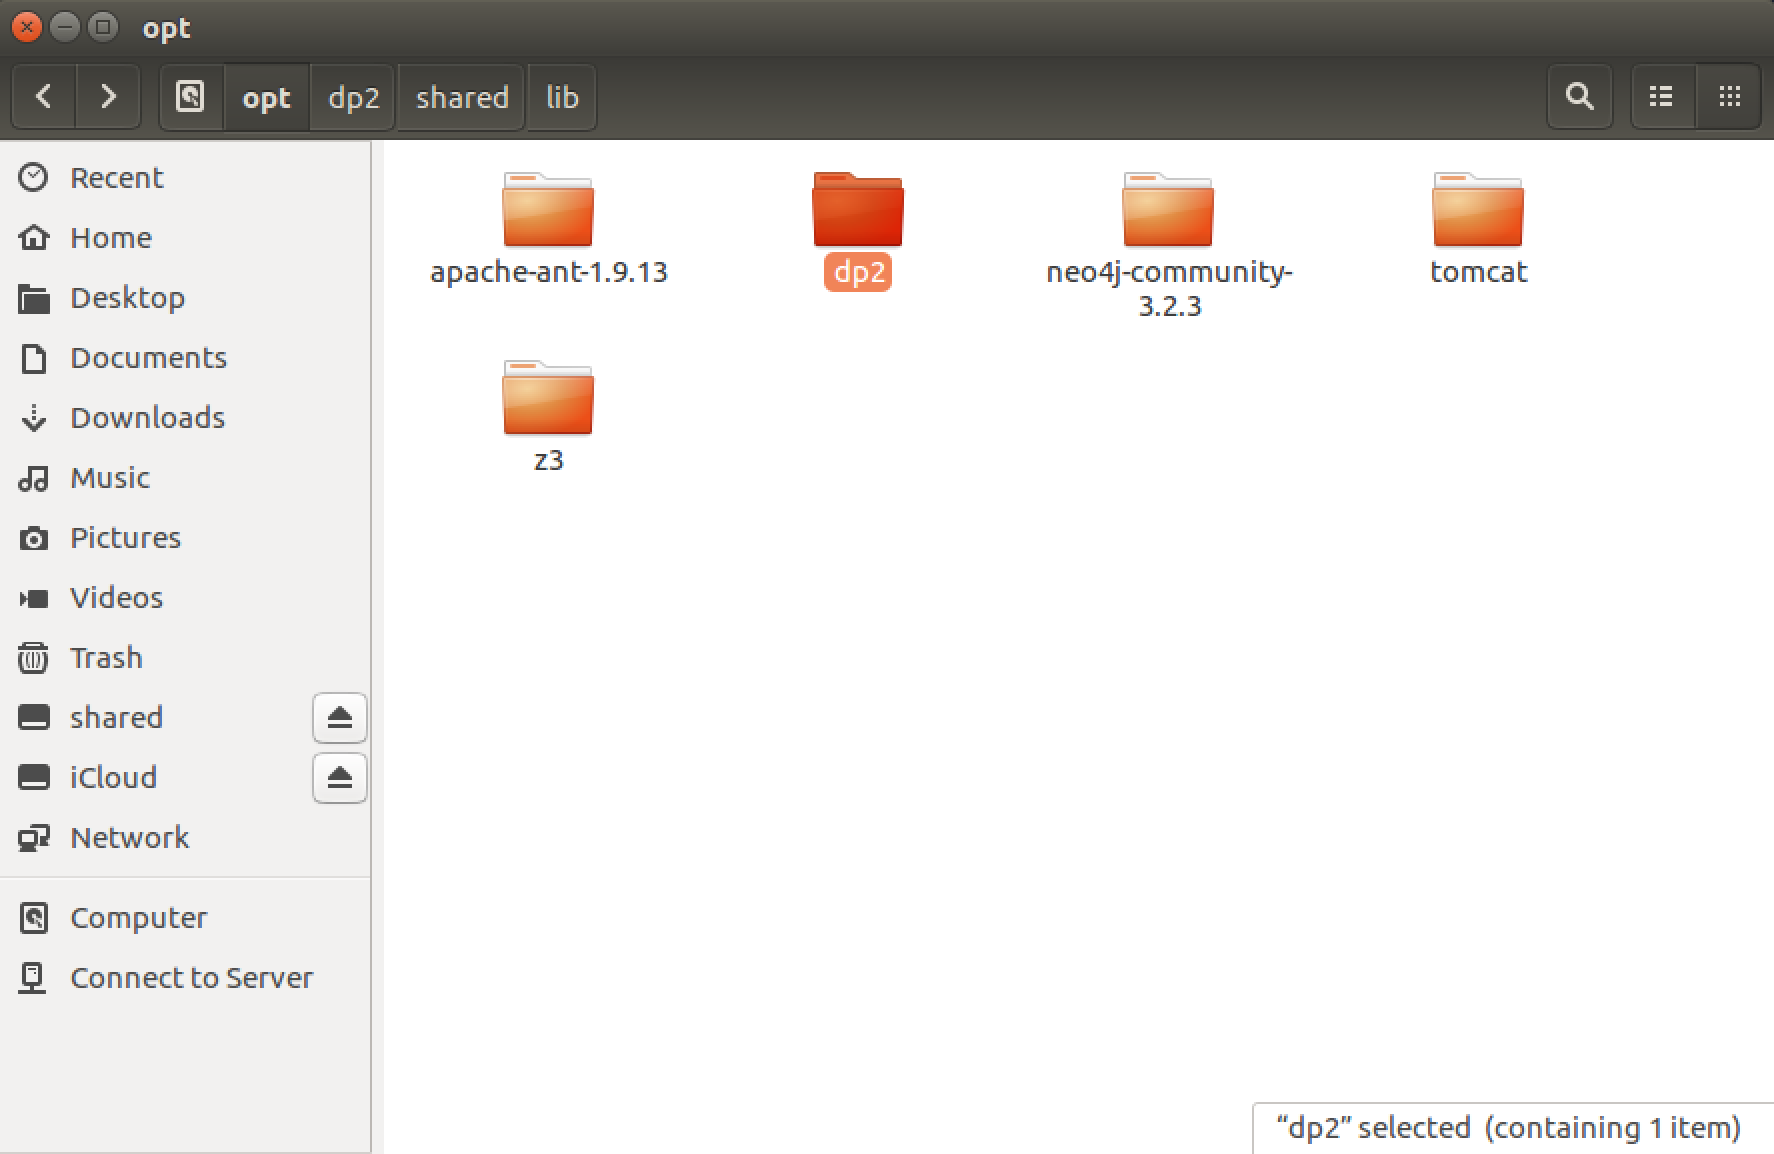
\includegraphics[width=\textwidth]{opt_folder.png}
   \caption{Folder \textit{/opt} of the machine used as development environment.}\label{Fig:OptFolder}
\end{figure}
Additional library like neo4j drivers and junit are provided in the \textit{lib} and \textit{lib-src} folder of the application project. They are already included in classpath during compilation launched through ant scripts. If errors are signaled by Eclipse when opening the project, probably they should be added to build path. After the addition it is suggestable to refresh and clean the project.

\section{Server application and tests}
In order to launch and compile server application, tests and neo4j, a set of ant scripts. In particular:
\begin{itemize}
  \item ant script \textbf{neo4j-build.xml} provides a set of target to launch/stop/restart\&clean neo4j database;
  \item ant script \textbf{build.xml} provides all the target to start/stop tomcat, to deploy the application and to run tests, it relies upon another script to define the operation of such targets, that is \textbf{build-rns.xml}.
\end{itemize}
The targets can be either launched via Eclipse IDE or command line. \\
To setup the server up and running it is necessary to follow these step:
\begin{enumerate}
  \item start Neo4j by using \textbf{start-neo4j} target of \textbf{neo4j-build.xml} script. From command line \textit{ant 'start-neo4j' -f /path/to/neo4j-build.xml};
  \item start Tomcat by calling \textbf{start-tomcat} target of \textbf{build.xml} script. From command line \textit{ant 'start-tomcat' -f /path/to/build.xml};
  \item deploy web service by calling \textbf{redeploy} target of \textbf{build.xml} script. From command line \textit{ant 'redeploy' -f /path/to/build.xml}.
\end{enumerate}
This last command embed in itself the generation of the bindings from XML Schema with JAXB and the compilation of all the necessary classes.\\
In order to launch the tests written for the service it is necessary to use \textbf{rns-tests} target of \textbf{build.xml} script. This target will launch the coompilation of all the classes necessary to the tests and launch them with JUnit.
